\documentclass[11pt]{charter}

% El títulos de la memoria, se usa en la carátula y se puede usar el cualquier lugar del documento con el comando \ttitle
\titulo{Equipo adquisidor de descargas parciales} 

% Nombre del posgrado, se usa en la carátula y se puede usar el cualquier lugar del documento con el comando \degreename
\posgrado{Carrera de Especialización en Sistemas Embebidos} 
%\posgrado{Carrera de Especialización en Internet de las Cosas} 
%\posgrado{Carrera de Especialización en Intelegencia Artificial}
%\posgrado{Maestría en Sistemas Embebidos} 
%\posgrado{Maestría en Internet de las cosas}

% Tu nombre, se puede usar el cualquier lugar del documento con el comando \authorname
\autor{Pablo Severini} 

% El nombre del director y co-director, se puede usar el cualquier lugar del documento con el comando \supname y \cosupname y \pertesupname y \pertecosupname
\director{Dr. Ing. Marcos Maillot}
\pertenenciaDirector{UTN FRGP} 
% FIXME:NO IMPLEMENTADO EL CODIRECTOR ni su pertenencia
\codirector{Ing. Cristian Bonini} % si queda vacio no se deberíá incluir 
\pertenenciaCoDirector{UTN FRGP}

% Nombre del cliente, quien va a aprobar los resultados del proyecto, se puede usar con el comando \clientename y \empclientename
\cliente{Marcos Maillot}
\empresaCliente{UTN FRGP}

% Nombre y pertenencia de los jurados, se pueden usar el cualquier lugar del documento con el comando \jurunoname, \jurdosname y \jurtresname y \perteunoname, \pertedosname y \pertetresname.
\juradoUno{Nombre y Apellido (1)}
\pertenenciaJurUno{pertenencia (1)} 
\juradoDos{Nombre y Apellido (2)}
\pertenenciaJurDos{pertenencia (2)}
\juradoTres{Nombre y Apellido (3)}
\pertenenciaJurTres{pertenencia (3)}
 
\fechaINICIO{22 de junio de 2020}		%Fecha de inicio de la cursada de GdP \fechaInicioName
\fechaFINALPlanificacion{22 de Agosto de 2020} 	%Fecha de final de cursada de GdP
\fechaFINALTrabajo{22 de Agosto de 2021}		%Fecha de defensa pública del trabajo final


\begin{document}

\maketitle
\thispagestyle{empty}
\pagebreak


\thispagestyle{empty}
{\setlength{\parskip}{0pt}
\tableofcontents{}
}
\pagebreak


\section{Registros de cambios}
\label{sec:registro}


\begin{table}[ht]
\label{tab:registro}
\centering

\begin{tabularx}{\linewidth}{@{}|c|X|c|@{}}
\hline
\rowcolor[HTML]{C0C0C0} 
Revisión & \multicolumn{1}{c|}{\cellcolor[HTML]{C0C0C0}Detalles de los cambios realizados} & Fecha      \\ \hline
1.0      & 	Creación del documento     							& 22/06/2020 \\ \hline
1.1      & 	Se agrega del punto 1 al 6	 						& 05/07/2020 \\ \hline
1.2      & 	Se agregan las correcciones del punto 1 al 6		& 15/07/2020 \\ \hline
1.3      & 	Se agrega del punto 7 al 11							& 23/07/2020 \\ \hline
\end{tabularx}
\end{table}

\pagebreak



\section{Acta de Constitución del Proyecto}
\label{sec:acta}

\begin{flushright}
Buenos Aires, \fechaInicioName
\end{flushright}

\vspace{2 cm}

Por medio de la presente se acuerda con el Ing. \authorname\hspace{1px} que su Trabajo Final de la \degreename\hspace{1px} se titulará ``\ttitle'', consistirá esencialmente en un equipo que detecte pulsos de descargas parciales traducidos por un sensor externo y mediante la referencia de la fase bajo medición construya un patrón de descargas parciales. Tendrá un presupuesto preliminar estimado de 800\euro\ y 600 hs de trabajo, con fecha de inicio \fechaInicioName\hspace{1px} y fecha de presentación pública \fechaFinalName.

Se adjunta a esta acta la planificación inicial.

\vfill

% Esta parte se construye sola con la información que hayan cargado en el preámbulo del documento y no debe modificarla
\begin{table}[ht]
\centering
\begin{tabular}{ccc}
\begin{tabular}[c]{@{}c@{}}Ariel Lutenberg \\ Director posgrado FIUBA\end{tabular} &  & \begin{tabular}[c]{@{}c@{}}\clientename \\ \empclientename \end{tabular} \vspace{2.5cm} \\ 
\begin{tabular}[c]{@{}c@{}}\supname \\ Director del Trabajo Final\end{tabular} &  & 
\begin{tabular}[c]{@{}c@{}}\cosupname \\ Co-Director del Trabajo Final \end{tabular} \vspace{2.5cm} \\ 
\begin{tabular}[c]{@{}c@{}}\jurunoname \\ Jurado del Trabajo Final\end{tabular}     &  & \begin{tabular}[c]{@{}c@{}}\jurdosname\\ Jurado del Trabajo Final\end{tabular}  \vspace{2.5cm}  \\
\multicolumn{3}{c}{\begin{tabular}[c]{@{}c@{}} \jurtresname\\ Jurado del Trabajo Final\end{tabular}} \vspace{.5cm}                                                                     
\end{tabular}
\end{table}




\section{Descripción técnica-conceptual del Proyecto a realizar}
\label{sec:descripcion}

Introducción general al tema

Una descarga parcial es un fenómeno de disrupción eléctrica. Se caracteriza por ser un
pulso de corriente de alta frecuencia el cual se produce en el seno de un sistema aislante de
una máquina o equipo eléctrico de potencia como consecuencia de la presencia de
oclusiones gaseosas, impurezas, aristas aguzadas u otras anomalías que distorsionan la
distribución de las líneas de campo eléctrico.

La ocurrencia de este fenómeno provoca un deterioro local del sistema aislante. Indistintamente de cuál sea el medio en
el que este fenómeno se manifiesta y cual sea la causa que lo origina, el deterioro del
sistema es acumulativo.

El generador de patrones de descargas parciales (en adelante DP) es un equipo que permite realizar mediciones de
distintos tipos de DP en máquinas o equipos eléctricos de potencia. Por medio de estas
mediciones es posible monitorear el estado de su aislación.
En la figura 1 se presenta el diagrama en bloques del sistema.

\begin{figure}[htpb]
\centering 
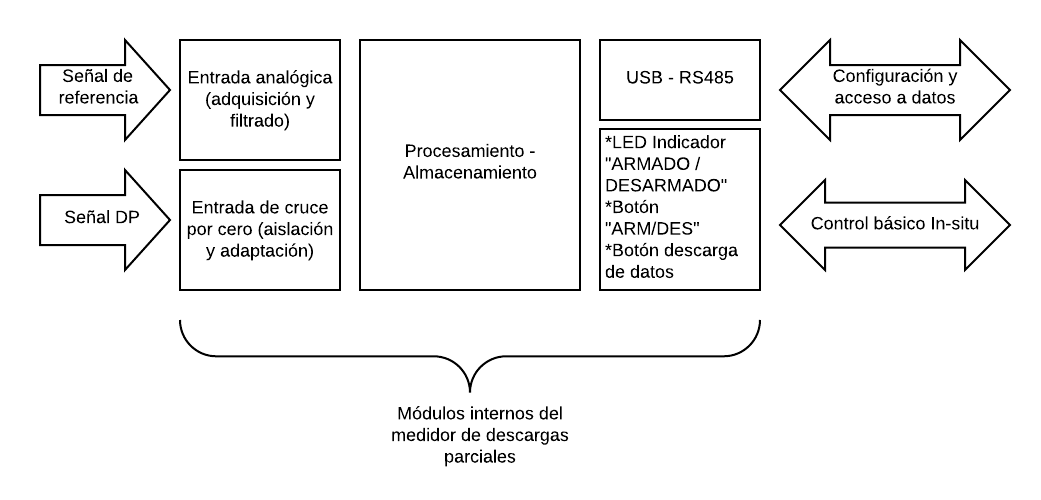
\includegraphics[width=1\textwidth]{./Figuras/diagBloques1.png}
\caption{Diagrama en bloques del sistema}
\label{fig:diagBloques}
\end{figure}

Descripción detallada

El objetivo del presente trabajo es desarrollar un sistema capaz de detectar los picos
máximos de los pulsos de DP y representarlos sobre una senoide de referencia de
frecuencia industrial - 50 Hertz – en fase con la tensión de ensayo. La superposición de
eventos conformará una nube cuya estructura o morfología dará indicios del tipo de DP
(corona, interna o superficial).
A la representación antes mencionada se la conoce con el nombre de “Patrón de DP”. Una
imagen de este puede apreciarse en la figura 2.

\begin{figure}[H]
\centering 
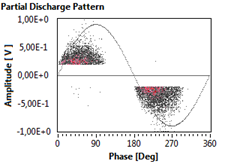
\includegraphics[width=.5\textwidth]{./Figuras/patronDP.png}
\caption{Ejemplo de patrón de DP del tipo interna}
\label{fig:diagBloques}
\end{figure}


Estado del arte

Actualmente existen equipos de medición de descargas parciales fabricados por empresas extranjeras como TechImp, PD Power Diagnostic, Omnicrom. El sistema propuesto se diferencia de los antes mencionados por ser un equipo de bajo costo capaz de ser instalado de forma fija para realizar monitoreo en tiempo real.


\section{Identificación y análisis de los interesados}
\label{sec:interesados}

\begin{table}[ht]
%\caption{Identificación de los interesados}
%\label{tab:interesados}
\begin{tabularx}{\linewidth}{@{}|l|X|X|l|@{}}
\hline
\rowcolor[HTML]{C0C0C0} 
Rol           & Nombre y Apellido & Organización 	& Puesto 	\\ \hline
Cliente       & \clientename      &\empclientename	& Director	Trabajo final       	\\ \hline
Impulsor      & \authorname       & FIUBA         	& Alumno   	\\ \hline
Responsable   & \authorname       & FIUBA        	& Alumno 	\\ \hline
Orientador    & \cosupname 		  & \pertesupname 	& Co-Director	Trabajo final \\ \hline
\end{tabularx}
\end{table}


\section{1. Propósito del proyecto}
\label{sec:proposito}

El propósito de este proyecto es crear un equipo de medición de descargas parciales de bajo costo capaz de ser instalado permanentemente, para brindar un monitoreo constante, rápido y eficiente.

\section{2. Alcance del proyecto}
\label{sec:alcance}

El presente proyecto incluye:
\begin{itemize}
\item El desarrollo del prototipo del producto.
\item El desarrollo del firmware.
\item El diseño electrónico del hardware.
\item Confección de un manual de uso.
\item Pruebas de validación y verificación.
\end{itemize}

El presente proyecto no incluye:
\begin{itemize}
\item El desarrollo del equipo final.
\item Diseño de gabinete.
\item Pruebas en campo.
\end{itemize}


\section{3. Supuestos del proyecto}
\label{sec:supuestos}

\begin{itemize}
\item UTN FRGP proveerá una base de datos de señales de DP adquiridas sobre distintas probetas de distintos materiales dieléctricos en laboratorio. 
\item En el ámbito del COVID 2019, no se cerrarán las importaciones impidiendo el acceso a equipamiento o materiales necesarios para la ejecución del proyecto.
\end{itemize}

\section{4. Requerimientos}
\label{sec:requerimientos}

\begin{enumerate}
\item Requerimientos generales
	\begin{enumerate}
	\item El dispositivo deberá, mediante el procesamiento de las adquisiciones, detectar los picos máximos de los pulsos de DP y representarlos sobre una senoide de referencia de frecuencia industrial - 50 Hertz - en fase con la tensión de ensayo (generar un patrón de DP).
	\item El dispositivo deberá funcionar como un sistema \textit{"stand-alone"}.
	\item El dispositivo debe mantener la fecha y hora por medio de un RTC.
	\item El dispositivo deberá tener un puerto de acceso serial (preferentemente diferencial) para configuración y acceso a datos remoto.
	\item El dispositivo deberá contar con un puerto USB para la descarga de los patrones de DP.
	\end{enumerate}
\item Requerimientos asociados a la configuración
	\begin{enumerate}
	\item El dispositivo deberá permitir modificar el umbral de disparo a partir del cual se comenzará a procesar una señal.
	\item El dispositivo deberá permitir modificar la cantidad de muestras que serán procesadas por disparo (máximo 1000).
	\item El dispositivo deberá permitir modificar la cantidad de disparos (máximo 1000) que componen a un patrón de DP.
	\item El dispositivo deberá permitir configurar el RTC.
	\item El dispositivo deberá permitir planificar la generación automática de un patrón DP cada periodos múltiplos de 1 hora (calendario).
	\item El dispositivo deberá permitir generar un patrón de DP con los parámetros configurados a demanda y transferirlo por el puerto serie.
	\end{enumerate}
\item Requerimientos asociados al modo de trabajo
	\begin{enumerate}
	\item El dispositivo deberá permitir poner al sistema en modo “ARMADO” y “ DESARMADO”.
	\item En modo “ARMADO” el dispositivo deberá cumplir con las adquisiciones preestablecidas por calendario.
	\item En modo “DESARMADO” el dispositivo no estará operativo.
	\end{enumerate}
\item Requerimientos asociados a la adquisición de la señal de referencia
	\begin{enumerate}
	\item La entrada de señal de referencia debe poder detectar los cruces por cero de una senoide de 50 Hz, y saber su polaridad.
	\item La entrada de señal de referencia debe ser opto-acoplada.
	\item El dispositivo deberá llevar un contador en milisegundos a partir de la señal de cruce por cero. De forma tal que se pueda saber en todo momento si está transcurriendo un semiciclo positivo o negativo y saber cuánto tiempo transcurrió desde su inicio.
	\end{enumerate}
\item Requerimientos asociados a la adquisición de la señal analógica
	\begin{enumerate}
	\item Se deben poder adquirir señales con una ancho de banda entre 0.1MHz y 40Mhz con una resolución mínima de 8 bits.
	\item La amplitud máxima de la señal de entrada sera de 1 Vpp.
	\item La entrada para el sensor analógico deberá ser de 50 ohms diferencial.
 	\item El dispositivo deberá detectar cuando la señal muestreada supere el umbral de disparo, si esto sucediera las siguientes muestras (cantidad definida anteriormente en la configuración) deberán ser comparadas entre sí y preservar la de mayor magnitud. El valor obtenido deberá ser almacenado en memoria, junto con un \textit{timestamp}, la polaridad del semiciclo de referencia y su momento angular. Este proceso debe ser repetido hasta que se cumplan los disparos que componen un patrón DP.
	\end{enumerate}
\item Requerimientos asociados a la interfaz de usuario
	\begin{enumerate}
	\item Deberá indicará su estado “ARMADO - DESARMADO” por medio de un led de estado.
	\item Deberá permitir “ARMAR - DESARMAR” al sistema por medio de una tecla física.
	\item Deberá realizar la acción de transferir a un \textit{pendrive} el contenido total de la memoria interna por medio de una tecla física.
	\end{enumerate}
\item Requerimientos de acceso a datos
	\begin{enumerate}
	\item El dispositivo deberá listar todos los patrones de DP almacenados bajo el siguiente identificador “AAMMDDhhmm” en base a la fecha de generación del patrón. 
	\item El dispositivo deberá permitir seleccionar al patrón por medio de su identificador y solicitar su transferencia por puerto serie.
	\end{enumerate}

\end{enumerate}

\section{5. Entregables principales del proyecto}
\label{sec:entregables}

\begin{itemize}
\item Manual de uso
\item Diagrama esquemático
\item Diagrama de instalación
\item \textit{Firmware}
\item Informe final

\end{itemize}

\section{6. Desglose del trabajo en tareas}
\label{sec:wbs}

\begin{enumerate}
\item Planificación
	\begin{enumerate}
	\item Realizar el plan de proyecto (20 hs)
	\end{enumerate}
\item Recopilación de información
	\begin{enumerate}
	\item Búsqueda de información teórica de muestreo a alta velocidad (32 hs)
	\item Búsqueda de componentes para la etapa de adquisición analógica (26 hs)
	\end{enumerate}
\item Diseño de y validación del \textit{hardware}
	\begin{enumerate}
	\item Selección y cálculo de filtros. (10 hs)
	\item Diseño del esquemático para la etapa de adquisición analógica. (20 hs)
	\item Diseño del \textit{PCB} para la etapa de adquisición analógica. (12 hs)
	\item Montaje de componentes. (8 hs)
	\item Verificación y puesta en marcha del \textit{hardware}. (20 hs)
	\item Validación de la etapa analógica por medio de inyección señales. (15 hs)
	\item Codificar funciones para validar el diseño de la adquisición analógica. (30 hs)
	\end{enumerate}
\item Desarrollo módulo de adquisición
	\begin{enumerate}
	\item Codificar funciones de comunicación con ADC. (40 hs)
	\item Codificar funciones de detección de cruce por cero. (15 hs)
	\item Codificar funciones para el umbral de disparo. (24 hs)
	\end{enumerate}
\item Desarrollo módulos auxiliares
	\begin{enumerate}
	\item Codificar funciones de comunicación para la UART. (30 hs)
	\item Codificar funciones del reloj de tiempo real. (20 hs)
	\item Codificar funciones de botones de entrada y led de estado. (4 hs)
	\item Codificar funciones de almacenamiento USB. (40 hs)
	\end{enumerate}
\item Integración
	\begin{enumerate}
	\item Integrar todos los módulos de software. (50 hs) 	
	\item Pruebas funcionales.	(30 hs)
	\item Integrar los módulos de funciones de adquisición. (50 hs)
	\end{enumerate}
\item Proceso final
	\begin{enumerate}
	\item Confeccionar manual de uso. (10 hs) 	
	\item Confeccionar memoria (50 hs)
	\item Revisión final del documento (24 hs)
	\item Diseño del esquemático final.	(20 hs)
	\end{enumerate}
\end{enumerate}

Cantidad total de horas: (600 hs)


\begin{landscape}

\section{7. Diagrama de Activity On Node}
\label{sec:AoN}

\begin{figure}[htpb]
\centering 
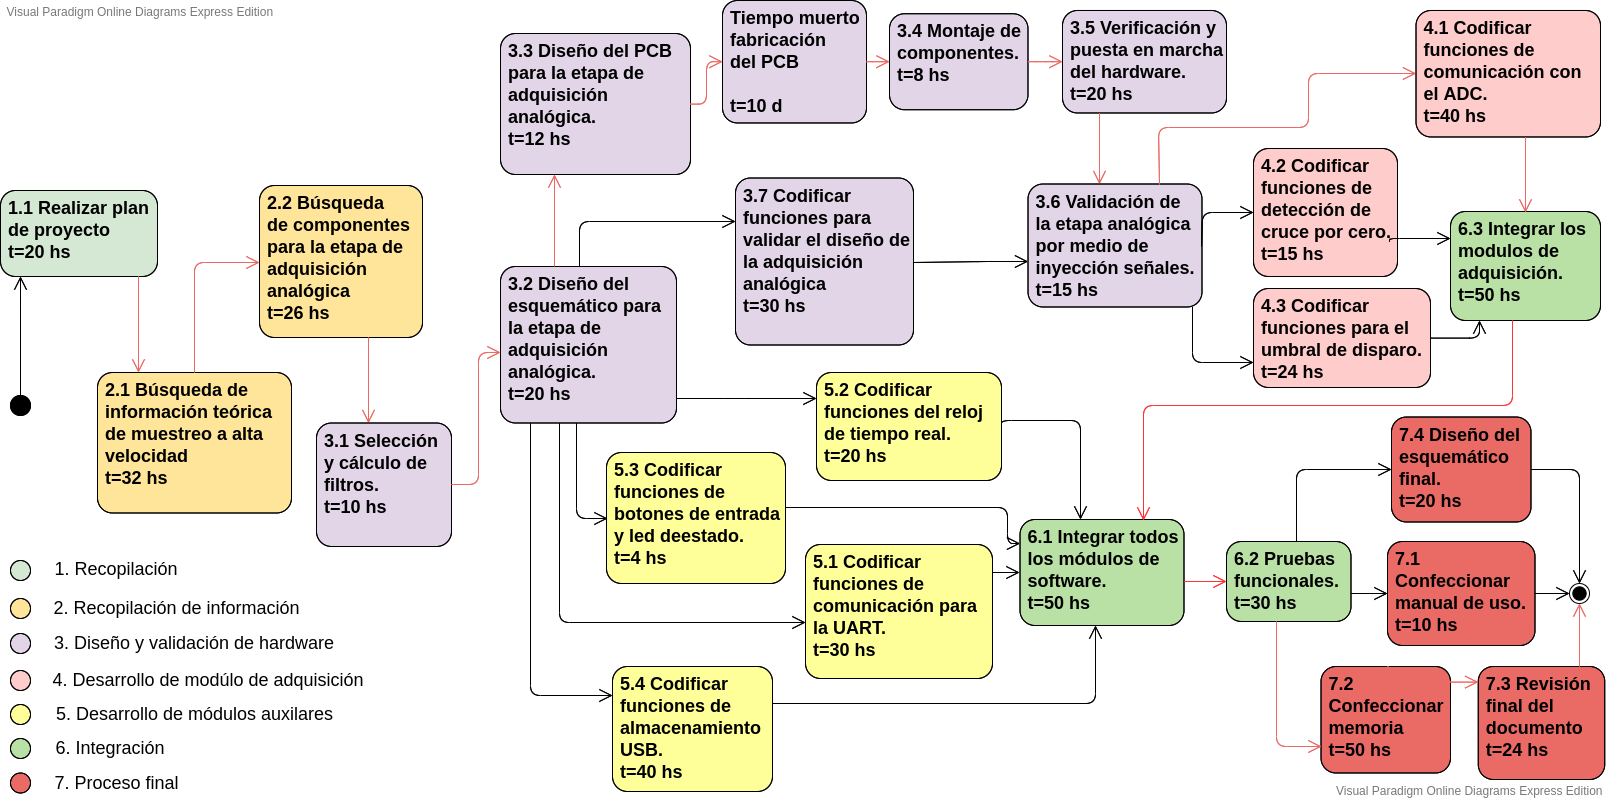
\includegraphics[width=1.6\textwidth]{./Figuras/AON.png}
\caption{Diagrama en \textit{Activity on Node}}
\label{fig:AoN}
\end{figure}
\end{landscape}

\section{8. Diagrama de Gantt}
\label{sec:gantt}

\begin{figure}[htpb]
\centering 
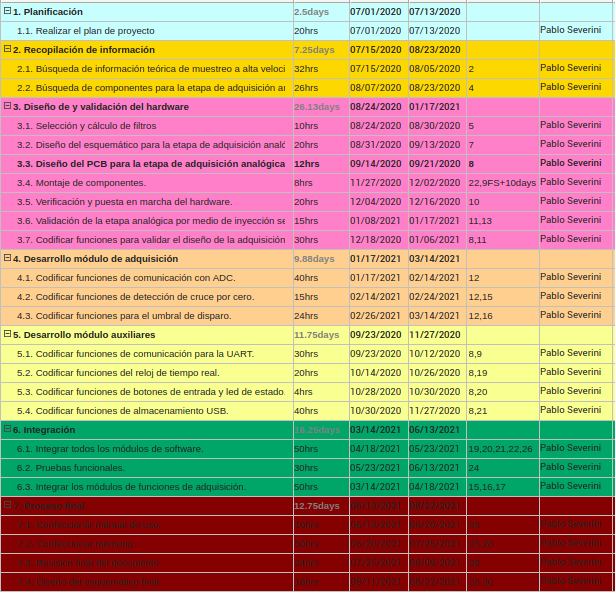
\includegraphics[width=1\textwidth]{./Figuras/tablaGant.png}
\caption{Tareas Gantt}
\label{fig:AoN}
\end{figure}

\begin{landscape}
\begin{figure}[htpb]
\centering 
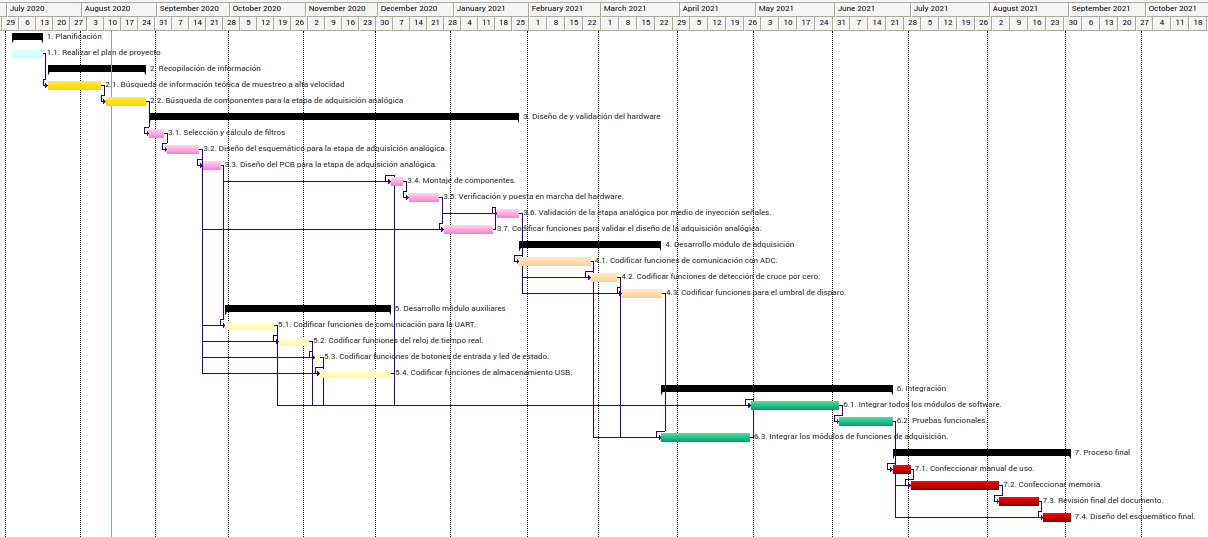
\includegraphics[width=1.6\textwidth]{./Figuras/calendarioGant.png}
\caption{Calendario Gantt}
\label{fig:AoN}
\end{figure}
\end{landscape}


\section{9. Matriz de uso de recursos de materiales}
\label{sec:recursos}
\begin{table}[H]
\centering
\resizebox{\textwidth}{!}{%
\begin{tabular}{|c|c|c|c|c|c|}
\hline
\rowcolor[HTML]{C0C0C0} 
\cellcolor[HTML]{C0C0C0} &
  \cellcolor[HTML]{C0C0C0} &
  \multicolumn{4}{c|}{\cellcolor[HTML]{C0C0C0}Recursos requeridos (horas)} \\ \cline{3-6} 
\rowcolor[HTML]{C0C0C0} 
\multirow{-3}{*}{\cellcolor[HTML]{C0C0C0}\begin{tabular}[c]{@{}c@{}}Código WBS\end{tabular}} &
  \multirow{-3}{*}{\cellcolor[HTML]{C0C0C0}Nombre de la tarea} & PC & Placa digital & Placa analógica & Instrumentos \\ \hline
\multicolumn{6}{|c|}{\cellcolor[HTML]{7ACFF5}1. Planificacion} \\ \hline
1.1 & Realizar el plan de proyecto & 16 hs &  &  &    \\ \hline  
\multicolumn{6}{|c|}{\cellcolor[HTML]{FFE599}2. Recopilación de información} \\ \hline
2.1 & Búsqueda de información teórica de muestreo a alta velocidad & 32 hs &  &  &    \\ \hline
2.2 & Búsqueda de componentes para la etapa de adquisición analógica & 30 hs &  &  &    \\ \hline
\multicolumn{6}{|c|}{\cellcolor[HTML]{C3ABD0}3 Diseño de y validación del \textit{hardware}} \\ \hline
3.1 & Selección y cálculo de filtros. & 10 hs &  &  &    \\ \hline
3.2 & Diseño del esquemático para la etapa de adquisición analógica. & 20 hs &  &  &    \\ \hline
3.3 & Diseño del \textit{PCB} para la etapa de adquisición analógica. & 12 hs &  &  &    \\ \hline
3.4 & Montaje de componentes. &  &  & 8 hs &    \\ \hline
3.5 & Verificación y puesta en marcha del \textit{hardware}. &  &  & 20 hs & 20 hs  \\ \hline
3.6 & Validación de la etapa analógica por medio de inyección señales. &  &  & 15 hs & 15 hs   \\ \hline
3.7 & Codificar funciones para validar el diseño de la adquisición analógica. & 30 hs & 30 hs &  &   \\ \hline
\multicolumn{6}{|c|}{\cellcolor[HTML]{FF3333}4 Desarrollo módulo de adquisición} \\ \hline
4.1 & Codificar funciones de comunicación con ADC. & 40 hs & 40 hs &  &    \\ \hline
4.2 & Codificar funciones de detección de cruce por cero. & 15 hs & 15 hs &  & 5 hs   \\ \hline
4.3 & Codificar funciones para el umbral de disparo. & 24 hs & 24 hs &  &  5 hs  \\ \hline
\multicolumn{6}{|c|}{\cellcolor[HTML]{FFFF00}5 Desarrollo módulo auxiliares} \\ \hline
5.1 & Codificar funciones de comunicación para la UART. & 30 hs & 30 hs &  &    \\ \hline
5.2 & Codificar funciones del reloj de tiempo real. & 20 hs & 20 hs &  &    \\ \hline
5.3 & Codificar funciones de botones de entrada y led de estado. & 4 hs & 4 hs &  &    \\ \hline
5.4 & Codificar funciones de almacenamiento USB. & 40 hs & 40 hs &  &    \\ \hline
\multicolumn{6}{|c|}{\cellcolor[HTML]{66CC00}6 Integración} \\ \hline
6.1 & Integrar todos los módulos de software. & 50 hs & 30 hs & 30 hs & 10 hs   \\ \hline
6.2 & Pruebas funcionales. & 30 hs & 30 hs & 30 hs & 30 hs   \\ \hline
6.3 & Integrar los módulos de funciones de adquisición. & 50 hs & 50 hs & 50 hs & 50 hs  \\ \hline
\multicolumn{6}{|c|}{\cellcolor[HTML]{EA6B66}7 Proceso final} \\ \hline
7.1 & Confeccionar manual de uso. & 10 hs &  &  &    \\ \hline
7.2 & Confeccionar memoria. & 50 hs &  &  &    \\ \hline
7.3 & Revisión final del documento. & 24 hs &  &  &    \\ \hline
7.4 & Diseño del esquemático final. & 20 hs &  &  &    \\ \hline  
\rowcolor[HTML]{C0C0C0} 
\multicolumn{2}{|c|}{\cellcolor[HTML]{C0C0C0} Totales} & 539 hs & 295 hs & 153 hs & 135 hs    \\ \hline
\end{tabular}%
}
\end{table}

\section{10. Presupuesto detallado del proyecto}
\label{sec:presupuesto}

\begin{table}[htpb]
\centering
\begin{tabularx}{\linewidth}{@{}|X|c|r|r|@{}}
\hline
\rowcolor[HTML]{C0C0C0} 
\multicolumn{4}{|c|}{\cellcolor[HTML]{C0C0C0}COSTOS DIRECTOS} \\ \hline
\rowcolor[HTML]{C0C0C0} 
Descripción &
  \multicolumn{1}{c|}{\cellcolor[HTML]{C0C0C0}Cantidad} &
  \multicolumn{1}{c|}{\cellcolor[HTML]{C0C0C0}Valor unitario} &
  \multicolumn{1}{c|}{\cellcolor[HTML]{C0C0C0}Valor total} \\ \hline
 Modulo K210 Maix Dock&
  \multicolumn{1}{c|}{1} &
  \multicolumn{1}{c|}{25\euro} &
  \multicolumn{1}{c|}{25\euro} \\ \hline
 PCB&
  \multicolumn{1}{c|}{1} &
  \multicolumn{1}{c|}{25\euro} &
  \multicolumn{1}{c|}{25\euro} \\ \hline
 Componentes etapa analógica&
  \multicolumn{1}{c|}{1} &
  \multicolumn{1}{c|}{100\euro} &
  \multicolumn{1}{c|}{100\euro} \\ \hline
\multicolumn{3}{|c|}{SUBTOTAL} &
  \multicolumn{1}{c|}{150\euro} \\ \hline
\rowcolor[HTML]{C0C0C0} 
\multicolumn{4}{|c|}{\cellcolor[HTML]{C0C0C0}COSTOS INDIRECTOS} \\ \hline
\rowcolor[HTML]{C0C0C0} 
Descripción &
  \multicolumn{1}{c|}{\cellcolor[HTML]{C0C0C0}Cantidad} &
  \multicolumn{1}{c|}{\cellcolor[HTML]{C0C0C0}Valor unitario} &
  \multicolumn{1}{c|}{\cellcolor[HTML]{C0C0C0}Valor total} \\ \hline
 Osciloscopio Siglent SDS1202X-E &
  \multicolumn{1}{c|}{1} &
  \multicolumn{1}{c|}{365\euro} &
  \multicolumn{1}{c|}{365\euro} \\ \hline
 Generador de onda arbitraria DDS FY6900 &
  \multicolumn{1}{c|}{1} &
  \multicolumn{1}{c|}{85\euro} &
  \multicolumn{1}{c|}{85\euro} \\ \hline
 Fuente de laboratorio Minleaf NPS3010W &
  \multicolumn{1}{c|}{1} &
  \multicolumn{1}{c|}{40\euro} &
  \multicolumn{1}{c|}{40\euro} \\ \hline
 Cables y adaptadores SMA a BNC &
  \multicolumn{1}{c|}{1} &
  \multicolumn{1}{c|}{20\euro} &
  \multicolumn{1}{c|}{20\euro} \\ \hline
\multicolumn{3}{|c|}{SUBTOTAL} &
  \multicolumn{1}{c|}{510\euro} \\ \hline
\rowcolor[HTML]{C0C0C0}
\multicolumn{3}{|c|}{TOTAL} & 660\euro
   \\ \hline
\end{tabularx}%
\end{table}
(*)Valores aproximados

\section{11. Matriz de asignación de responsabilidades}
\label{sec:responsabilidades}

\begin{table}[H]
\centering
\resizebox{\textwidth}{!}{%
\begin{tabular}{|c|c|c|c|c|c|}
\hline
\rowcolor[HTML]{C0C0C0} 
\cellcolor[HTML]{C0C0C0} &
  \cellcolor[HTML]{C0C0C0} &
  \multicolumn{3}{c|}{\cellcolor[HTML]{C0C0C0}Listar todos los nombres y roles del proyecto} \\ \cline{3-5} 
\rowcolor[HTML]{C0C0C0} 
\cellcolor[HTML]{C0C0C0} &
  \cellcolor[HTML]{C0C0C0} &
  Responsable &
  Orientador &
  Cliente \\ \cline{3-5} 
\rowcolor[HTML]{C0C0C0} 
\multirow{-3}{*}{\cellcolor[HTML]{C0C0C0}\begin{tabular}[c]{@{}c@{}}Código\\ WBS\end{tabular}} &
  \multirow{-3}{*}{\cellcolor[HTML]{C0C0C0}Nombre de la tarea} &
  \authorname &
  \cosupname &
  \clientename \\ \hline
\multicolumn{5}{|c|}{\cellcolor[HTML]{7ACFF5}1. Planificacion} \\ \hline
1.1 & Realizar el plan de proyecto & P & I & A   \\ \hline  
\multicolumn{5}{|c|}{\cellcolor[HTML]{FFE599}2. Recopilación de información} \\ \hline
2.1 & Búsqueda de información teórica de muestreo a alta velocidad & P & C & I   \\ \hline
2.2 & Búsqueda de componentes para la etapa de adquisición analógica & P & C & I   \\ \hline
\multicolumn{5}{|c|}{\cellcolor[HTML]{C3ABD0}3 Diseño de y validación del \textit{hardware}} \\ \hline
3.1 & Selección y cálculo de filtros. & P & C & C   \\ \hline
3.2 & Diseño del esquemático para la etapa de adquisición analógica. & P & I & I   \\ \hline
3.3 & Diseño del \textit{PCB} para la etapa de adquisición analógica. & P & I & I   \\ \hline
3.4 & Montaje de componentes. & P & - & -   \\ \hline
3.5 & Verificación y puesta en marcha del \textit{hardware}. & P & I & I  \\ \hline
3.6 & Validación de la etapa analógica por medio de inyección señales. & P & I & I   \\ \hline
3.7 & Codificar funciones para validar el diseño de la adquisición analógica. & P & - & -  \\ \hline
\multicolumn{5}{|c|}{\cellcolor[HTML]{FF3333}4 Desarrollo módulo de adquisición} \\ \hline
4.1 & Codificar funciones de comunicación con ADC. & P & - & -   \\ \hline
4.2 & Codificar funciones de detección de cruce por cero. & P & - & -   \\ \hline
4.3 & Codificar funciones para el umbral de disparo. & P & - & -   \\ \hline
\multicolumn{5}{|c|}{\cellcolor[HTML]{FFFF00}5 Desarrollo módulo auxiliares} \\ \hline
5.1 & Codificar funciones de comunicación para la UART. & P & - & -   \\ \hline
5.2 & Codificar funciones del reloj de tiempo real. & P & - & -  \\ \hline
5.3 & Codificar funciones de botones de entrada y led de estado. & P & - & -   \\ \hline
5.4 & Codificar funciones de almacenamiento USB. & P & - & -   \\ \hline
\multicolumn{5}{|c|}{\cellcolor[HTML]{66CC00}6 Integración} \\ \hline
6.1 & Integrar todos los módulos de software. & P & I & I   \\ \hline
6.2 & Pruebas funcionales. & P & C & A  \\ \hline
6.3 & Integrar los módulos de funciones de adquisición. & P & I & I  \\ \hline
\multicolumn{5}{|c|}{\cellcolor[HTML]{EA6B66}7 Proceso final} \\ \hline
7.1 & Confeccionar manual de uso. & P & I & A   \\ \hline
7.2 & Confeccionar memoria. & P & C & A   \\ \hline
7.3 & Revisión final del documento. & P & C & A   \\ \hline
7.4 & Diseño del esquemático final. & P & I & I   \\ \hline  
\end{tabular}%
}
\end{table}

{\footnotesize
Referencias:
\begin{itemize}
	\item P = Responsabilidad Primaria
	\item S = Responsabilidad Secundaria
	\item A = Aprobación
	\item I = Informado
	\item C = Consultado
\end{itemize}
} %footnotesize

\section{12. Gestión de riesgos}
\label{sec:riesgos}

\begin{consigna}{red}
a) Identificación de los riesgos (al menos cinco) y estimación de sus consecuencias:
 
Riesgo 1: detallar el riesgo (riesgo es algo que si ocurre altera los planes previstos)
\begin{itemize}
\item Severidad (S): mientras más severo, más alto es el número (usar números del 1 al 10).\\
Justificar el motivo por el cual se asigna determinado número de severidad (S).
\item Probabilidad de ocurrencia (O): mientras más probable, más alto es el número (usar del 1 al 10).\\
Justificar el motivo por el cual se asigna determinado número de (O). 
\end{itemize}   

Riesgo 2:
\begin{itemize}
\item Severidad (S): 
\item Ocurrencia (O):
\end{itemize}

Riesgo 3:
\begin{itemize}
\item Severidad (S): 
\item Ocurrencia (O):
\end{itemize}


b) Tabla de gestión de riesgos:      (El RPN se calcula como RPN=SxO)

\begin{table}[htpb]
\centering
\begin{tabularx}{\linewidth}{@{}|X|c|c|c|c|c|c|@{}}
\hline
\rowcolor[HTML]{C0C0C0} 
Riesgo & S & O & RPN & S* & O* & RPN* \\ \hline
       &   &   &     &    &    &      \\ \hline
       &   &   &     &    &    &      \\ \hline
       &   &   &     &    &    &      \\ \hline
       &   &   &     &    &    &      \\ \hline
       &   &   &     &    &    &      \\ \hline
\end{tabularx}%
\end{table}

Criterio adoptado: 
Se tomarán medidas de mitigación en los riesgos cuyos números de RPN sean mayores a ....

Nota: los valores marcados con (*) en la tabla corresponden luego de haber aplicado la mitigación.

c) Plan de mitigación de los riesgos que originalmente excedían el RPN máximo establecido:
 
Riesgo 1: Plan de mitigación (si por el RPN fuera necesario elaborar un plan de mitigación).
  Nueva asignación de S y O, con su respectiva justificación:
  - Severidad (S): mientras más severo, más alto es el número (usar números del 1 al 10).
          Justificar el motivo por el cual se asigna determinado número de severidad (S).
  - Probabilidad de ocurrencia (O): mientras más probable, más alto es el número (usar del 1 al 10).
          Justificar el motivo por el cual se asigna determinado número de (O).

Riesgo 2: Plan de mitigación (si por el RPN fuera necesario elaborar un plan de mitigación).
 
Riesgo 3: Plan de mitigación (si por el RPN fuera necesario elaborar un plan de mitigación)

\end{consigna}


\section{13. Gestión de la calidad}
\label{sec:calidad}

\begin{consigna}{red}
Para cada uno de los requerimientos del proyecto indique:
\begin{itemize} 
\item Req \#1: Copiar acá el requerimiento.

Verificación y validación:

\begin{itemize}
\item Verificación para confirmar si se cumplió con lo requerido antes de mostrar el sistema al cliente:\\
Detallar 
\item Validación con el cliente para confirmar que está de acuerdo en que se cumplió con lo requerido:\\
Detallar  
\end{itemize}

\end{itemize}

Tener en cuenta que en este contexto se pueden mencionar simulaciones, cálculos, revisión de hojas de datos, consulta con expertos, etc.

\end{consigna}

\section{14. Comunicación del proyecto}
\label{sec:comunicaciones}

\begin{consigna}{red}
El plan de comunicación del proyecto es el siguiente:
\end{consigna}

% Please add the following required packages to your document preamble:
% \usepackage{graphicx}
% \usepackage[table,xcdraw]{xcolor}
% If you use beamer only pass "xcolor=table" option, i.e. \documentclass[xcolor=table]{beamer}
\begin{table}[htpb]
\centering
\resizebox{\textwidth}{!}{%
\begin{tabular}{|c|c|c|c|c|c|}
\hline
\rowcolor[HTML]{C0C0C0} 
\multicolumn{6}{|c|}{\cellcolor[HTML]{C0C0C0}PLAN DE COMUNICACIÓN DEL PROYECTO}           \\ \hline
\rowcolor[HTML]{C0C0C0} 
¿Qué comunicar? & Audiencia & Propósito & Frecuencia & Método de comunicac. & Responsable \\ \hline
                &           &           &            &                      &             \\ \hline
                &           &           &            &                      &             \\ \hline
                &           &           &            &                      &             \\ \hline
                &           &           &            &                      &             \\ \hline
                &           &           &            &                      &             \\ \hline
\end{tabular}%
}
\end{table}

\section{15. Gestión de Compras}
\label{sec:compras}

\begin{consigna}{red}
En caso de tener que comprar elementos o contratar servicios:
a) Explique con qué criterios elegiría a un proveedor.
b) Redacte el Statement of Work correspondiente.
\end{consigna}

\section{16. Seguimiento y control}
\label{sec:seguimiento}

\begin{consigna}{red}
Para cada tarea del proyecto establecer la frecuencia y los indicadores con los se seguirá su avance y quién será el responsable de hacer dicho seguimiento y a quién debe comunicarse la situación (en concordancia con el Plan de Comunicación del proyecto).

El indicador de avance tiene que ser algo medible, mejor incluso si se puede medir en \% de avance. Por ejemplo,se pueden indicar en esta columna cosas como ``cantidad de conexiones ruteadeas'' o ``cantidad de funciones implementadas'', pero no algo genérico y ambiguo como ``\%'', porque el lector no sabe porcentaje de qué cosa.

\end{consigna}

\begin{table}[!htpb]
\centering
\begin{tabularx}{\linewidth}{@{}|X|X|X|X|X|X|@{}}
\hline
\rowcolor[HTML]{C0C0C0} 
\multicolumn{6}{|c|}{\cellcolor[HTML]{C0C0C0}SEGUIMIENTO DE AVANCE}                                                                       \\ \hline
\rowcolor[HTML]{C0C0C0} 
Tarea del WBS & Indicador de avance & Frecuencia de reporte & Resp. de seguimiento & Persona a ser informada & Método de comunic. \\ \hline
 &  &  &  &  &  \\ \hline
 &  &  &  &  &  \\ \hline
 &  &  &  &  &  \\ \hline
 &  &  &  &  &  \\ \hline
 &  &  &  &  &  \\ \hline
\end{tabularx}%
%}
\end{table}

\section{17. Procesos de cierre}    
\label{sec:cierre}

\begin{consigna}{red}
Establecer las pautas de trabajo para realizar una reunión final de evaluación del proyecto, tal que contemple las siguientes actividades:

\begin{itemize}
\item Pautas de trabajo que se seguirán para analizar si se respetó el Plan de Proyecto original:
 - Indicar quién se ocupará de hacer esto y cuál será el procedimiento a aplicar. 
\item Identificación de las técnicas y procedimientos útiles e inútiles que se utilizaron, y los problemas que surgieron y cómo se solucionaron:
 - Indicar quién se ocupará de hacer esto y cuál será el procedimiento para dejar registro.
\item Indicar quién organizará el acto de agradecimiento a todos los interesados, y en especial al equipo de trabajo y colaboradores:
  - Indicar esto y quién financiará los gastos correspondientes.
\end{itemize}

\end{consigna}


\end{document}
